\documentclass[12pt]{article}
\usepackage[landscape, margin=0.75in]{geometry}
\usepackage{booktabs}
\usepackage{longtable}
\usepackage{array}
\usepackage{graphicx}
\usepackage{enumitem}

\newcolumntype{C}[1]{>{\centering\arraybackslash}p{#1}}
\newcolumntype{L}[1]{>{\arraybackslash}p{#1}}

% Counter for question number column
\newcounter{qnum}
\setcounter{qnum}{0}
\newcommand{\nextq}{\stepcounter{qnum}\theqnum}

% Last column fills remaining width:
% Landscape letter = 11in, margins = 2x1in, so text = 9in
% Used: 1.5cm + 3cm + 7cm + 3x\tabcolsep*2 = 11.5cm + ~1cm = ~12.5cm
% Remaining ~ 9in - 12.5cm ~ 22.86cm - 12.5cm = ~10.36cm
\newlength{\qcol}
\setlength{\qcol}{10.36cm}

\begin{document}

\renewcommand{\arraystretch}{1.4}

\begin{longtable}{C{1.5cm} C{3cm} C{7cm} L{\qcol}}

% Header on first page
\toprule
\textbf{Question \#} & \textbf{Topic} & \textbf{Figure} & \textbf{Question Pool} \\
\midrule
\endfirsthead

% Header repeated on subsequent pages
\toprule
\textbf{Question \#} & \textbf{Topic} & \textbf{Figure} & \textbf{Question Pool} \\
\midrule
\endhead

% Footer on all pages except last
\midrule
\endfoot

% Footer on last page
\bottomrule
\endlastfoot

\nextq & Color Mapping
&
\raisebox{-0.9\height}{\includegraphics[width=6.5cm, height=4.5cm, keepaspectratio]{color-mapping/colormapping-surface-wallFilm.png}}
&
\begin{enumerate}[leftmargin=*, label=\arabic*., topsep=2pt, itemsep=6pt]
    \item What does the color represent in this image? 
\end{enumerate} \\

\midrule

\nextq & Color Mapping
&
\raisebox{-0.9\height}{\includegraphics[width=6.5cm, height=4cm, keepaspectratio]{color-mapping/color-map-remove-legend.png}}
&
\begin{enumerate}[leftmargin=*, label=\arabic*., topsep=2pt, itemsep=6pt]
    \item Given the following image, recommend one possible improvement.
\end{enumerate} \\

\midrule


\nextq & Glyphs
&
\raisebox{-0.9\height}{\includegraphics[width=6.5cm, height=5cm, keepaspectratio]{vector-glyphs/2D/glyph-2D-ring.png}}
&
\begin{enumerate}[leftmargin=*, label=\arabic*., topsep=2pt, itemsep=6pt]
    \item What type of vector field visualization technique is being used to convey flow in this figure?
    \item What do you think the size or the color of the glyphs in this image indicates?
\end{enumerate} \\

\midrule

\nextq & Glyphs
&
\raisebox{-0.9\height}{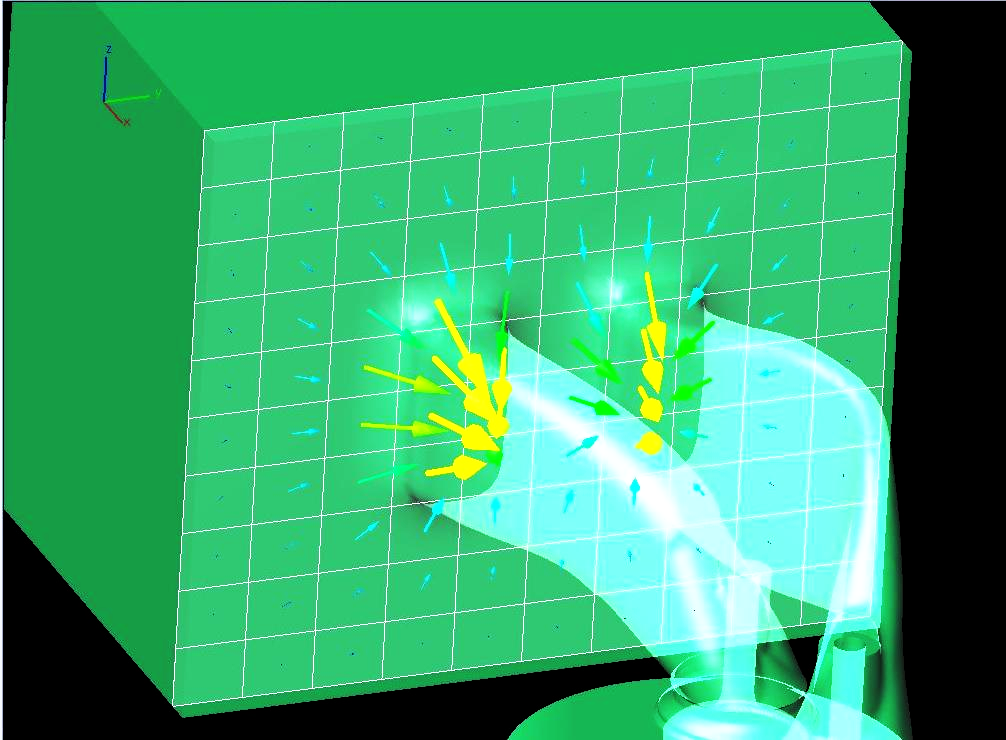
\includegraphics[width=6.5cm, height=4cm, keepaspectratio]{vector-glyphs/surface/glyph-surface-intake-resampled.png}}
&
\begin{enumerate}[leftmargin=*, label=\arabic*., topsep=2pt, itemsep=6pt]
    \item What type of vector field visualization is being used to convey flow in this figure?
    \item What do you think the size or the color of the glyphs in this image indicates?
    \item What kind of shapes do you see in this image to convey the characteristics of the flow?
    \item Where do you think the flow is the fastest in this figure?
\end{enumerate} \\

\midrule

\nextq & Glyphs
&
\raisebox{-0.9\height}{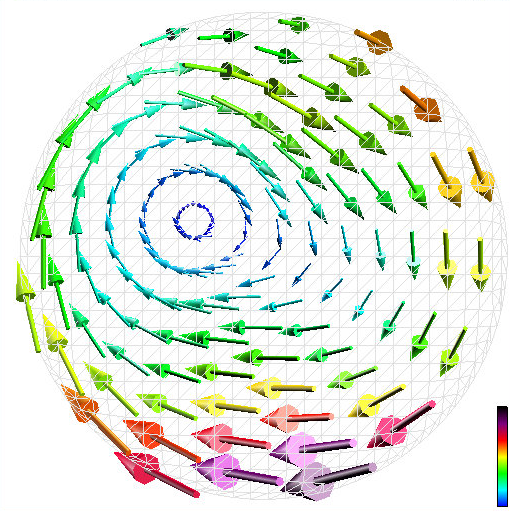
\includegraphics[width=6.5cm, height=4cm, keepaspectratio]{vector-glyphs/3D/glyphs-3D-slice.png}}
&
\begin{enumerate}[leftmargin=*, label=\arabic*., topsep=2pt, itemsep=6pt]
    \item Where in this figure is the upward flow? Please identify using the mouse pointer?
    \item What type of vector field visualization is being used to convey flow in this figure?
    \item What kind of shapes do you see in this image to convey the characteristics of the flow?
\end{enumerate} \\

\midrule

\nextq & Glyphs
&
\raisebox{-0.9\height}{\includegraphics[width=6.5cm, height=4cm, keepaspectratio]{vector-glyphs/3D/glyph-3D-resampled.png}}
&
\begin{enumerate}[leftmargin=*, label=\arabic*., topsep=2pt, itemsep=6pt]
    \item Where in this figure is the upward flow? Please identify using the mouse pointer?
    \item What type of vector field visualization is being used to convey flow in this figure?
    \item What kind of shapes do you see in this image to convey the characteristics of the flow?
\end{enumerate} \\



\midrule

\nextq & Streamlines
&
\raisebox{-0.9\height}{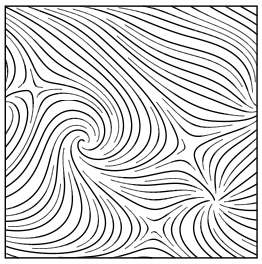
\includegraphics[width=6.5cm, height=4cm, keepaspectratio]{vector-streamlines/2D/streamlines.png}}
&
\begin{enumerate}[leftmargin=*, label=\arabic*., topsep=2pt, itemsep=6pt]
    \item What type of vector field visualization is being used to convey flow in this figure?
    \item How would you describe the spacing between the lines?
\end{enumerate} \\

\midrule

\nextq & Streamlines
&
\raisebox{-0.9\height}{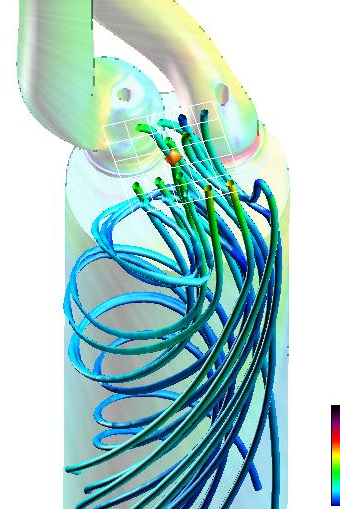
\includegraphics[width=6.5cm, height=4cm, keepaspectratio]{vector-streamlines/3D/streamlines-3D-intakePort.png}}
&
\begin{enumerate}[leftmargin=*, label=\arabic*., topsep=2pt, itemsep=6pt]
    \item What type of vector field visualization is being used to convey flow in this figure?
    \item How would you describe the shape of flow in this image? 
    \item What do you think color indicates in this figure? 
\end{enumerate} \\

\midrule

\nextq & Streamlines
&
\raisebox{-0.9\height}{\includegraphics[width=6.5cm, height=4cm, keepaspectratio]{vector-streamlines/3D/streamlines-3D-swirl.png}}
&
\begin{enumerate}[leftmargin=*, label=\arabic*., topsep=2pt, itemsep=6pt]
    \item What type of vector field visualization is being used to convey flow in this figure?
    \item How would you describe the direction of the flow field? 
\end{enumerate} \\


\midrule

\nextq & Streamlines
&
\raisebox{-0.9\height}{\includegraphics[width=6.5cm, height=4cm, keepaspectratio]{vector-streamlines/2D/hurricane38.png}}
&
\begin{enumerate}[leftmargin=*, label=\arabic*., topsep=2pt, itemsep=6pt]
    \item What type of vector field visualization is being used to convey flow in this figure?
    \item Click on a specific point in the image where you think the flow is separating
    \item Click on a specific location in the image, to identify a center point in the flow. 
\end{enumerate} \\

\midrule

\nextq & Texture-based
&
\raisebox{-0.9\height}{\includegraphics[width=6.5cm, height=4cm, keepaspectratio]{vector-texture-based/2D/texture-2D-gulf-2.png}}
&
\begin{enumerate}[leftmargin=*, label=\arabic*., topsep=2pt, itemsep=6pt]
    \item What type of vector field visualization is being used to convey flow in this figure?
    \item Locate one eddy current in the following image by clicking on the image.
\end{enumerate} \\

\midrule

\nextq & Texture-based
&
\raisebox{-0.9\height}{\includegraphics[width=6.5cm, height=4cm, keepaspectratio]{vector-texture-based/surface/texture-surface-intake.png}}
&
\begin{enumerate}[leftmargin=*, label=\arabic*., topsep=2pt, itemsep=6pt]
    \item What type of vector field visualization is being used to convey flow in this figure?
    \item Identify the application domain associated with this image.
    \item What is the dimensionality of the data conveyed in this image? 
\end{enumerate} \\

\midrule

\nextq & Texture-based
&
\raisebox{-0.9\height}{\includegraphics[width=6.5cm, height=4cm, keepaspectratio]{vector-texture-based/3D/texture-3D-wheel.png}}
&
\begin{enumerate}[leftmargin=*, label=\arabic*., topsep=2pt, itemsep=6pt]
    \item What type of vector field visualization is being used to convey flow in this figure?
    \item Identify the application domain associated with this image.
    \item What is the dimensionality of the data conveyed in this image? 
\end{enumerate} \\

\midrule

\nextq & Texture-based
&
\raisebox{-0.9\height}{\includegraphics[width=6.5cm, height=4cm, keepaspectratio]{vector-texture-based/surface/bmw.jpg}}
&
\begin{enumerate}[leftmargin=*, label=\arabic*., topsep=2pt, itemsep=6pt]
    \item What type of vector field visualization is being used to convey flow in this figure?
    \item Identify the application domain associated with this image.
    \item What is the dimensionality of the data conveyed in this image? 
\end{enumerate} \\

\midrule

\nextq & Tensor field visualization
&
\raisebox{-0.9\height}{
\includegraphics[width=6.5cm, height=4cm, keepaspectratio]{tensor/superquadrics.png}}
&
\begin{enumerate}[leftmargin=*, label=\arabic*., topsep=2pt, itemsep=6pt]
    \item What type of visualization technique is being used to represent the tensor field in this figure?
\end{enumerate} \\

\midrule

% \nextq & Tensor field visualization
% &
% \raisebox{-0.9\height}{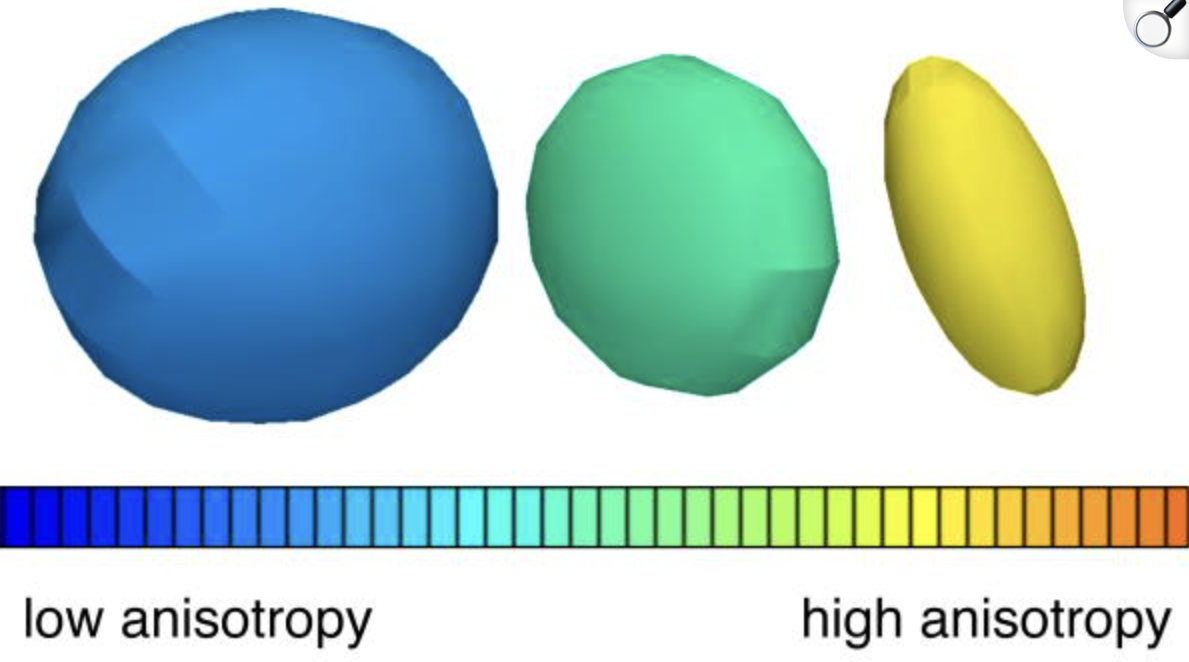
\includegraphics[width=6.5cm, height=4cm, keepaspectratio]{tensor/tensor-3x3.png}}
% &
% \begin{enumerate}[leftmargin=*, label=\arabic*., topsep=2pt, itemsep=6pt]
%     \item What is the dimensionality of the tensor field conveyed in this image? 
% \end{enumerate} \\

% \midrule

\nextq & Tensor field visualization
&
\raisebox{-0.9\height}{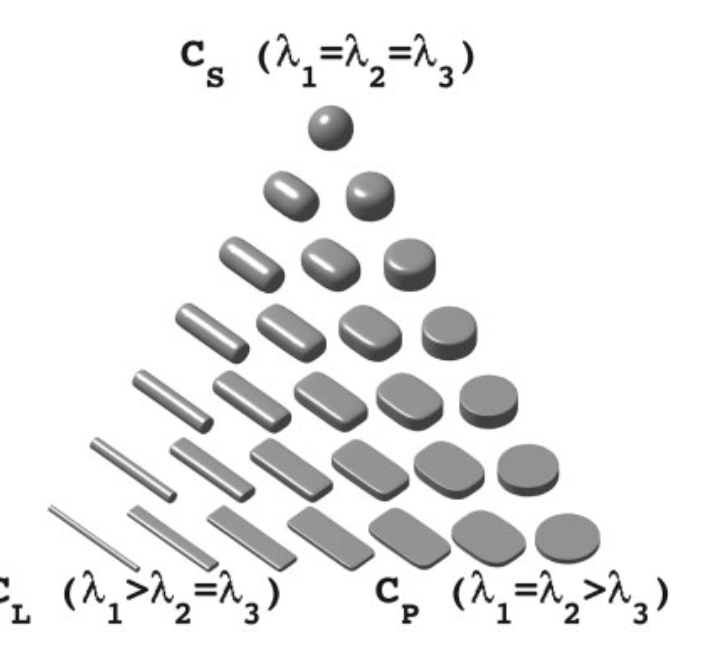
\includegraphics[width=6.5cm, height=4cm, keepaspectratio]{tensor/superquadrics-tensor.png}}
&
\begin{enumerate}[leftmargin=*, label=\arabic*., topsep=2pt, itemsep=6pt]
    \item What do the ellipsoid/superquadric shapes represent about the tensor data? 
\end{enumerate} \\

\midrule

\nextq & Tensor field visualization
&
\raisebox{-0.9\height}{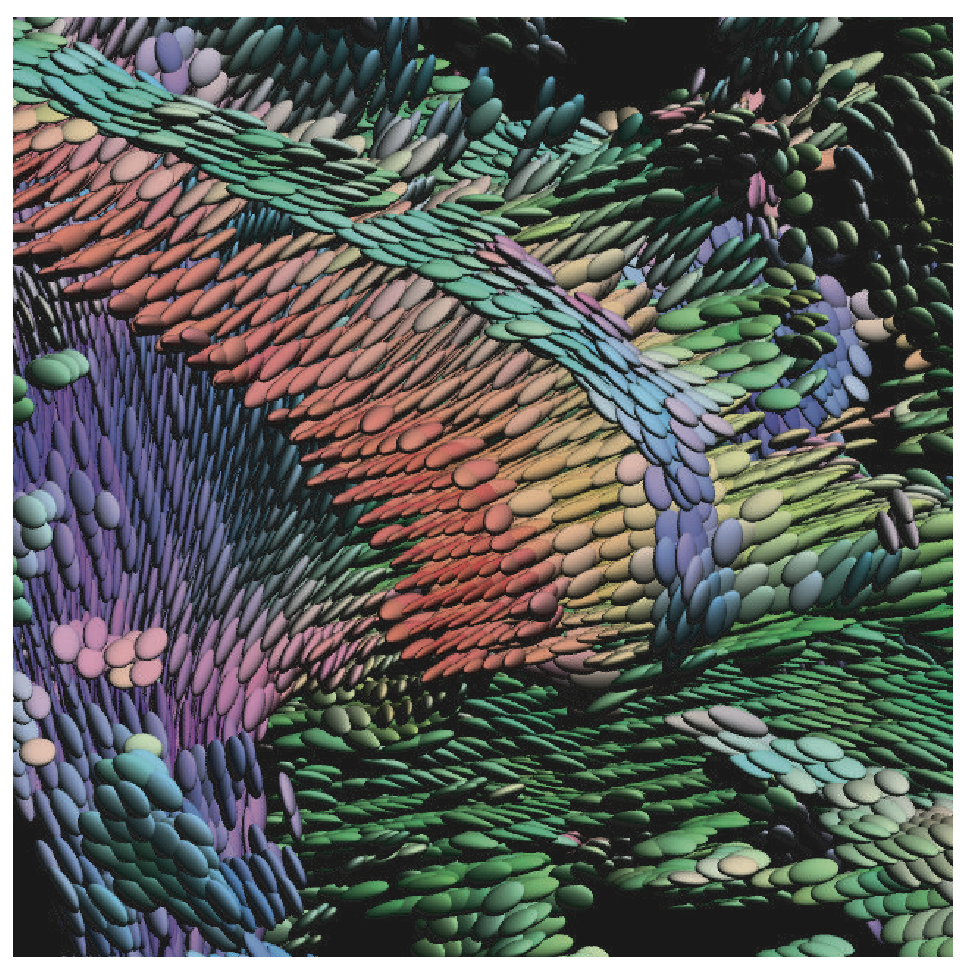
\includegraphics[width=6.5cm, height=4cm, keepaspectratio]{tensor/ellipsoid.png}}
&
\begin{enumerate}[leftmargin=*, label=\arabic*., topsep=2pt, itemsep=6pt]
    \item What type of glyph is used to represent the diffusion tensors in this DTI visualization? 
\end{enumerate} \\

\midrule

\nextq & Isolines \& Isocontours
&
\raisebox{-0.9\height}{\includegraphics[width=6.5cm, height=4cm, keepaspectratio]{scalar-isolines-isocontours/basic-contouring.png}}
&
\begin{enumerate}[leftmargin=*, label=\arabic*., topsep=2pt, itemsep=6pt]
    \item What type of visualization technique is used in this figure?
    \item What does the white line represent? 
\end{enumerate} \\

\midrule

\nextq & Isolines \& Isocontours
&
\raisebox{-0.9\height}{\includegraphics[width=6.5cm, height=4cm, keepaspectratio]{scalar-isolines-isocontours/Contours-of-a-temperature-map.png}}
&
\begin{enumerate}[leftmargin=*, label=\arabic*., topsep=2pt, itemsep=6pt]
    \item What type of visualization technique is used to generate this figure?
    \item What does the color red map to in the figure? 
\end{enumerate} \\

\midrule

\nextq & Isolines \& Isocontours
&
\raisebox{-0.9\height}{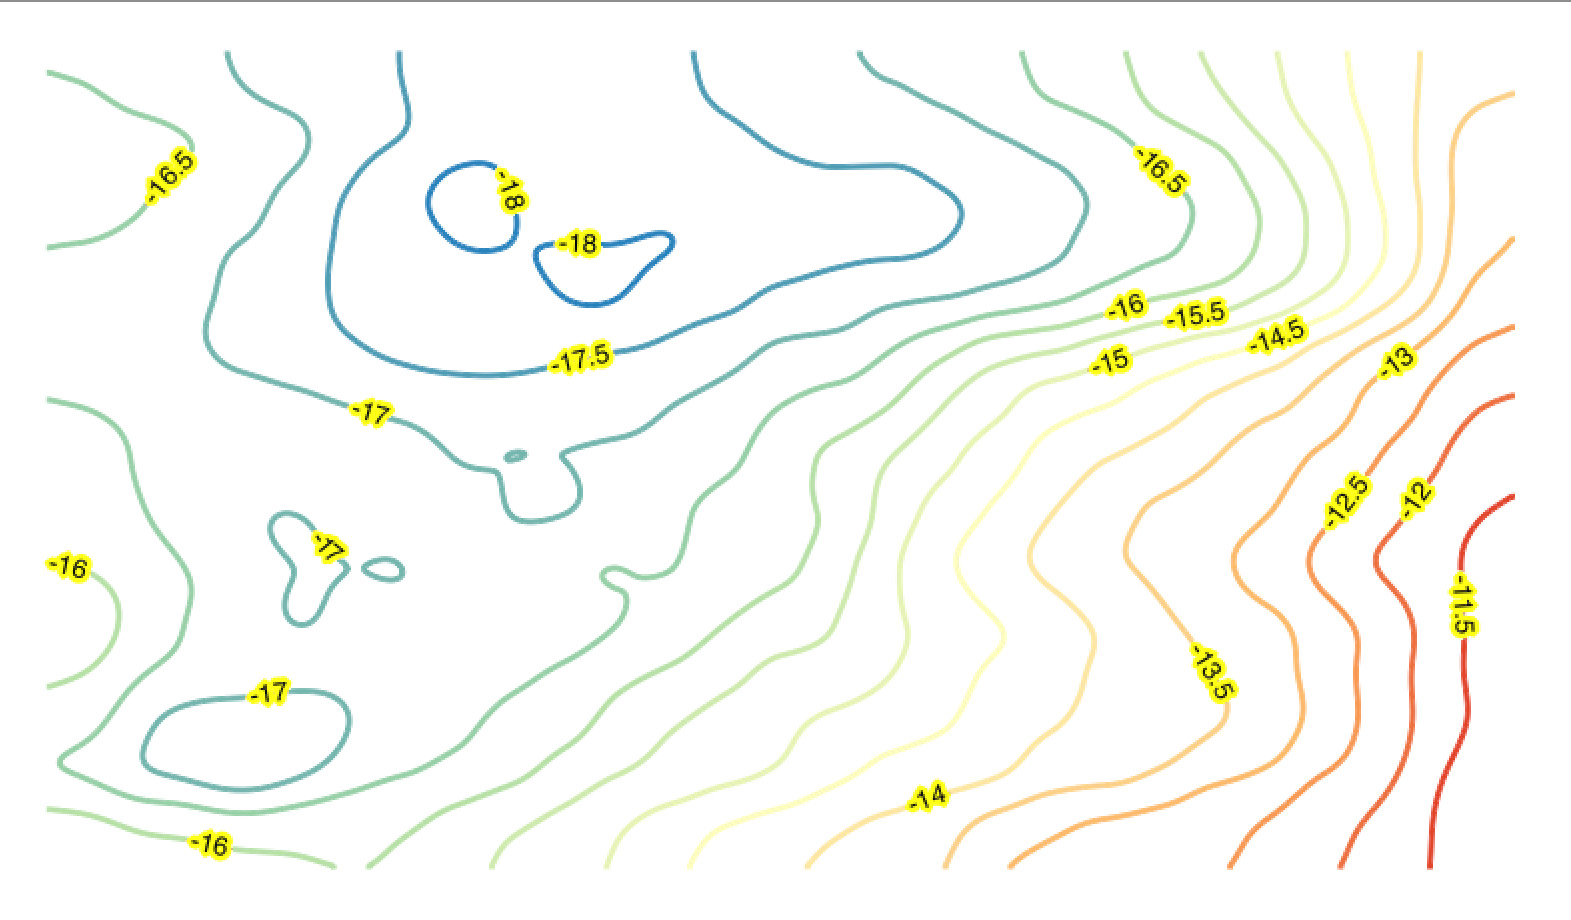
\includegraphics[width=6.5cm, height=4cm, keepaspectratio]{scalar-isolines-isocontours/isocontours.jpg}}
&
\begin{enumerate}[leftmargin=*, label=\arabic*., topsep=2pt, itemsep=6pt]
    \item What type of visualization technique is used to generate this figure?
    \item What do the colors represent in this image? 
\end{enumerate} \\

\midrule


\nextq & Isosurface Rendering
&
\raisebox{-0.9\height}{\includegraphics[width=6.5cm, height=4cm, keepaspectratio]{scalar-isosurface-rendering/isosurface5-vtkbook.png}}
&
\begin{enumerate}[leftmargin=*, label=\arabic*., topsep=2pt, itemsep=6pt]
    \item What type of visualization technique is used to generate this figure?
    \item What does the white color represent?  
    \item How many isosurface are rendered in this figure? 
\end{enumerate} \\

\midrule

\nextq & Isosurface Rendering
&
\raisebox{-0.9\height}{\includegraphics[width=6.5cm, height=4cm, keepaspectratio]{scalar-isosurface-rendering/lobster.png}}
&
\begin{enumerate}[leftmargin=*, label=\arabic*., topsep=2pt, itemsep=6pt]
    \item What type of visualization technique is used to generate this figure?
    \item What is the spatial dimensionality of the data used to generate this image? 
\end{enumerate} \\

\midrule

\nextq & Isosurface Rendering
&
\raisebox{-0.9\height}{\includegraphics[width=6.5cm, height=4cm, keepaspectratio]{scalar-isosurface-rendering/isosurface3-vtkbook.png}}
&
\begin{enumerate}[leftmargin=*, label=\arabic*., topsep=2pt, itemsep=6pt]
    \item What type of visualization technique is used to generate this figure?
    \item What is the spatial dimensionality of the data used to generate this image? 
\end{enumerate} \\

\midrule

\nextq & Volume Rendering
&
\raisebox{-0.9\height}{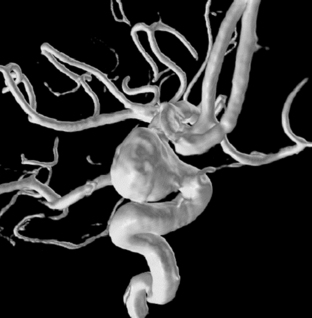
\includegraphics[width=6.5cm, height=4cm, keepaspectratio]{scalar-volume-rendering/volumeRendering-surface-handbook.jpg}}
&
\begin{enumerate}[leftmargin=*, label=\arabic*., topsep=2pt, itemsep=6pt]
    \item What type of visualization technique is used to generate this figure?
\end{enumerate} \\

\midrule

\nextq & Volume Rendering
&
\raisebox{-0.9\height}{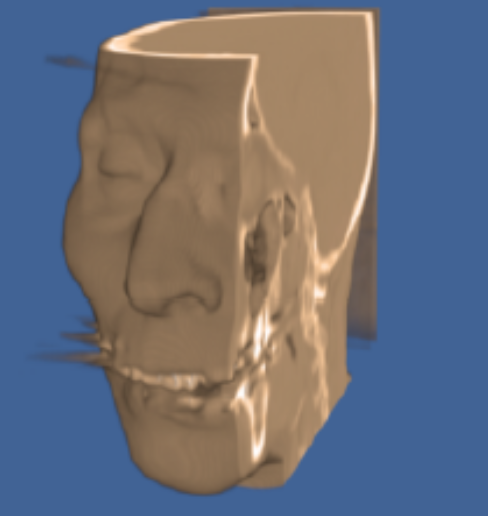
\includegraphics[width=6.5cm, height=4cm, keepaspectratio]{scalar-volume-rendering/texture-based-volren.png}}
&
\begin{enumerate}[leftmargin=*, label=\arabic*., topsep=2pt, itemsep=6pt]
    \item What type of visualization technique is used to generate this figure?
    \item Identify the application domain associated with this image.
\end{enumerate} \\

\midrule

\nextq & Volume Rendering
&
\raisebox{-0.9\height}{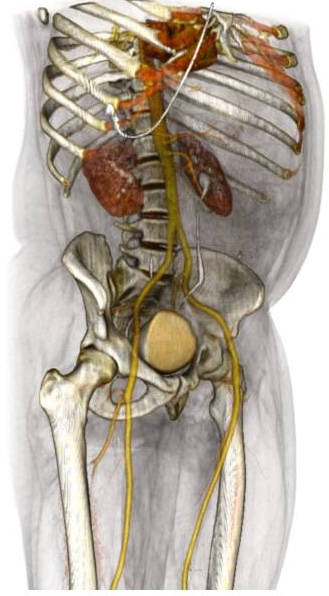
\includegraphics[width=6.5cm, height=4cm, keepaspectratio]{scalar-volume-rendering/occlusion-vr.jpg}}
&
\begin{enumerate}[leftmargin=*, label=\arabic*., topsep=2pt, itemsep=6pt]
    \item What type of visualization technique is used to generate this figure?
    \item What is the dimensionality of the data conveyed in this image? 
\end{enumerate} \\

\midrule

\nextq & Slicing \& Cutting 
&
\raisebox{-0.9\height}{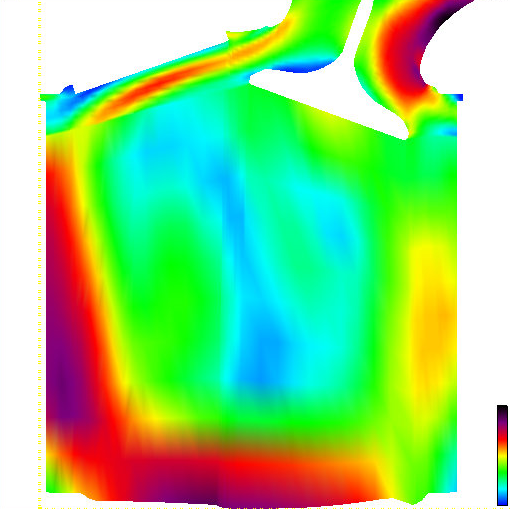
\includegraphics[width=6.5cm, height=4cm, keepaspectratio]{scalar-slicing-cutting/colormapping-2D-wallFilm.png}}
&
\begin{enumerate}[leftmargin=*, label=\arabic*., topsep=2pt, itemsep=6pt]
    \item What is the spatial dimensionality of this visualization technique used to generate this image? 
    \item Identify the application domain associated with this image. 
\end{enumerate} \\

\midrule

\nextq & Slicing \& Cutting 
&
\raisebox{-0.9\height}{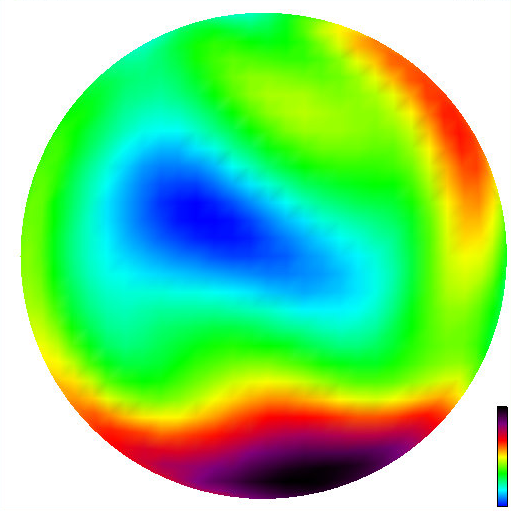
\includegraphics[width=6.5cm, height=4cm, keepaspectratio]{scalar-slicing-cutting/colormapping-2D-slice.png}}
&
\begin{enumerate}[leftmargin=*, label=\arabic*., topsep=2pt, itemsep=6pt]
    \item What is the dimensionality of the data conveyed in this image?  
    \item What do you think the color represents in this image? 
    \item What type of visualization technique is used in this image?  
\end{enumerate} \\

\midrule

\nextq & Slicing \& Cutting 
&
\raisebox{-0.9\height}{\includegraphics[width=6.5cm, height=4cm, keepaspectratio]{scalar-slicing-cutting/isosurfaces+slice.jpg}}
&
\begin{enumerate}[leftmargin=*, label=\arabic*., topsep=2pt, itemsep=6pt]
    \item What is the spatial dimensionality of the data used to generate this image?  
    \item Identify the application domain associated with this image.   
\end{enumerate} \\

\midrule


\nextq & Regular Grid
&
\raisebox{-0.9\height}{\includegraphics[width=6.5cm, height=4cm, keepaspectratio]{grid-regular/2D/rectilinear.png}}
&
\begin{enumerate}[leftmargin=*, label=\arabic*., topsep=2pt, itemsep=6pt]
    \item What type of grid is this? 
\end{enumerate} \\

\midrule

\nextq & Regular Grid
&
\raisebox{-0.9\height}{\includegraphics[width=6.5cm, height=4cm, keepaspectratio]{grid-regular/2D/anisotropic-rectilinear.png}}
&
\begin{enumerate}[leftmargin=*, label=\arabic*., topsep=2pt, itemsep=6pt]
    \item What type of grid is this? 
\end{enumerate} \\

\midrule

\nextq & Regular Grid
&
\raisebox{-0.9\height}{\includegraphics[width=6.5cm, height=4cm, keepaspectratio]{grid-regular/2D/rect-image.png}}
&
\begin{enumerate}[leftmargin=*, label=\arabic*., topsep=2pt, itemsep=6pt]
    \item What type of grid is this? 
\end{enumerate} \\

\midrule

\nextq & Regular Grid
&
\raisebox{-0.9\height}{\includegraphics[width=6.5cm, height=4cm, keepaspectratio]{grid-regular/2D/structured-circle.png}}
&
\begin{enumerate}[leftmargin=*, label=\arabic*., topsep=2pt, itemsep=6pt]
    \item What type of grid is this? 
\end{enumerate} \\


\midrule


\nextq & Curvilinear Grid
&
\raisebox{-0.9\height}{\includegraphics[width=6.5cm, height=4cm, keepaspectratio]{grid-curvilinear/2D/curvilinear.png}}
&
\begin{enumerate}[leftmargin=*, label=\arabic*., topsep=2pt, itemsep=6pt]
    \item What type of grid is this? 
\end{enumerate} \\

\midrule

\nextq & Curvilinear Grid
&
\raisebox{-0.9\height}{\includegraphics[width=6.5cm, height=4cm, keepaspectratio]{grid-curvilinear/3D/curvilinear.png}}
&
\begin{enumerate}[leftmargin=*, label=\arabic*., topsep=2pt, itemsep=6pt]
    \item What type of grid is this? 
\end{enumerate} \\

\midrule

\nextq & Unstructured Grid
&
\raisebox{-0.9\height}{\includegraphics[width=6.5cm, height=4cm, keepaspectratio]{grid-unstructured/2D/unstructured.png}}
&
\begin{enumerate}[leftmargin=*, label=\arabic*., topsep=2pt, itemsep=6pt]
    \item What type of grid is this? 
\end{enumerate} \\

\midrule

\nextq & Unstructured Grid
&
\raisebox{-0.9\height}{\includegraphics[width=6.5cm, height=4cm, keepaspectratio]{grid-curvilinear/3D/mesh-surface-unstructured-smaller.png}}
&
\begin{enumerate}[leftmargin=*, label=\arabic*., topsep=2pt, itemsep=6pt]
    \item What type of grid is this? 
\end{enumerate} \\

\midrule

\nextq & Medical
&
\raisebox{-0.9\height}{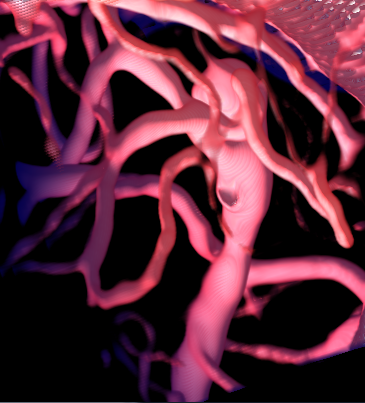
\includegraphics[width=6.5cm, height=4cm, keepaspectratio]{medical/3D/a_depth.png}}
&
\begin{enumerate}[leftmargin=*, label=\arabic*., topsep=2pt, itemsep=6pt]
    \item Identify the application domain associated with this image. 
    \item What is the dimensionality of the data conveyed in this image? 
\end{enumerate} \\

\midrule

\nextq & Medical
&
\raisebox{-0.9\height}{\includegraphics[width=6.5cm, height=4cm, keepaspectratio]{medical/surface/application-medical-wrist-surface-mip.png}}
&
\begin{enumerate}[leftmargin=*, label=\arabic*., topsep=2pt, itemsep=6pt]
    \item What do you think is being shown here? 
\end{enumerate} \\

\midrule

\nextq & Medical
&
\raisebox{-0.9\height}{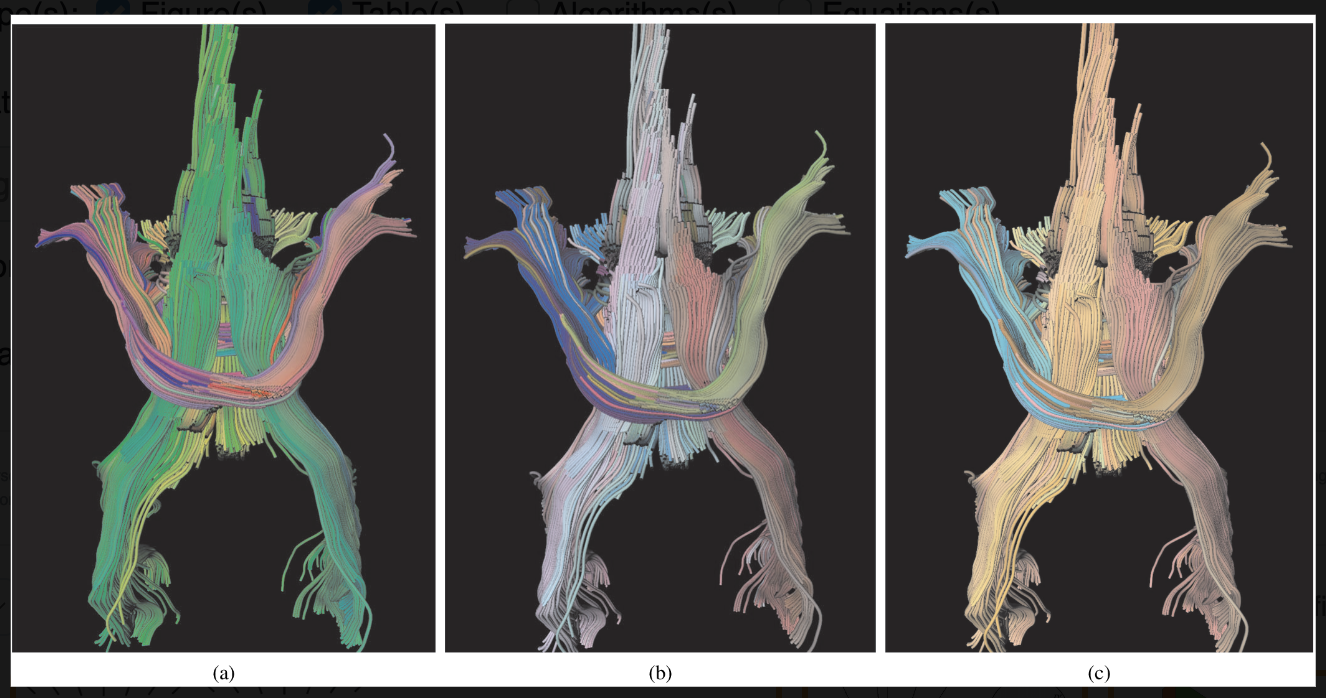
\includegraphics[width=6.5cm, height=4cm, keepaspectratio]{medical/3D/3D_ColorMapping.png}}
&
\begin{enumerate}[leftmargin=*, label=\arabic*., topsep=2pt, itemsep=6pt]
    \item Identify the medical visualization technique used to generate this figure? 
    \item What is the dimensionality of the data conveyed in this image? 
\end{enumerate} \\

\midrule

\nextq & Medical
&
\raisebox{-0.9\height}{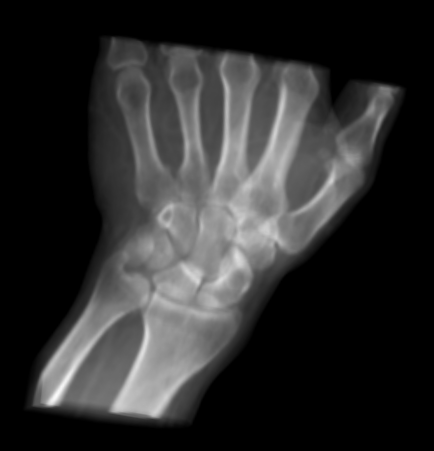
\includegraphics[width=6.5cm, height=4cm, keepaspectratio]{medical/3D/application-medical-wrist-3D-xray.png}}
&
\begin{enumerate}[leftmargin=*, label=\arabic*., topsep=2pt, itemsep=6pt]
    \item Identify the visualization technique used to generate this image. 
    \item What is the dimensionality of the data conveyed in this image? 
\end{enumerate} \\

\midrule

\nextq & Medical
&
\raisebox{-0.9\height}{\includegraphics[width=6.5cm, height=4cm, keepaspectratio]{medical/3D/hadwiger-007.png}}
&
\begin{enumerate}[leftmargin=*, label=\arabic*., topsep=2pt, itemsep=6pt]
    \item Identify the visualization technique used to generate this image. 
    \item What is the dimensionality of the data conveyed in this image? 
\end{enumerate} \\

\midrule

\nextq & Medical
&
\raisebox{-0.9\height}{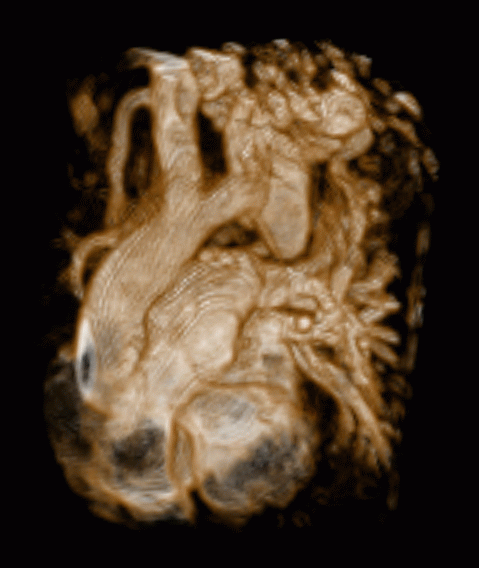
\includegraphics[width=6.5cm, height=4cm, keepaspectratio]{medical/3D/application-medical-heart.png}}
&
\begin{enumerate}[leftmargin=*, label=\arabic*., topsep=2pt, itemsep=6pt]
    \item Identify the application domain associated with this image. 
    \item What is the dimensionality of the data conveyed in this image? 
\end{enumerate} \\

\midrule


\nextq & Engineering \& CFD
&
\raisebox{-0.9\height}{\includegraphics[width=6.5cm, height=4cm, keepaspectratio]{engineering/surface/coolingjacket-surface-colorMapping-closeUp.png}}
&
\begin{enumerate}[leftmargin=*, label=\arabic*., topsep=2pt, itemsep=6pt]
    \item Identify the application domain associated with this image. 
    \item What is the dimensionality of the data conveyed in this image? 
\end{enumerate} \\

\midrule

\nextq & Engineering \& CFD
&
\raisebox{-0.9\height}{\includegraphics[width=6.5cm, height=4cm, keepaspectratio]{engineering/surface/coolingjacket-surface-isa.png}}
&
\begin{enumerate}[leftmargin=*, label=\arabic*., topsep=2pt, itemsep=6pt]
    \item What type of visualization technique is used to generate this figure?  
    \item What is the dimensionality of the data conveyed in this image? 
\end{enumerate} \\

\midrule

\nextq & Engineering \& CFD
&
\raisebox{-0.9\height}{\includegraphics[width=6.5cm, height=4cm, keepaspectratio]{engineering/3D/cylinder_topo_3d.png}}
&
\begin{enumerate}[leftmargin=*, label=\arabic*., topsep=2pt, itemsep=6pt]
    \item Identify the application domain associated with this image.
    \item What is the dimensionality of the data conveyed in this image? 
\end{enumerate} \\

\nextq & Molecular Dynamics
&
\raisebox{-0.9\height}{\includegraphics[width=6.5cm, height=4cm, keepaspectratio]{molecular-dynamics/2D/mdv.png}}
&
\begin{enumerate}[leftmargin=*, label=\arabic*., topsep=2pt, itemsep=6pt]
    \item Identify the application domain associated with this image.
\end{enumerate} \\

\midrule

\nextq & Molecular Dynamics
&
\raisebox{-0.9\height}{\includegraphics[width=6.5cm, height=4cm, keepaspectratio]{molecular-dynamics/3D/Zwan.2011.IMV-1.jpg}}
&
\begin{enumerate}[leftmargin=*, label=\arabic*., topsep=2pt, itemsep=6pt]
    \item What type of visualization technique is used to generate this figure? 
\end{enumerate} \\

\midrule

\nextq & Meteorology
&
\raisebox{-0.9\height}{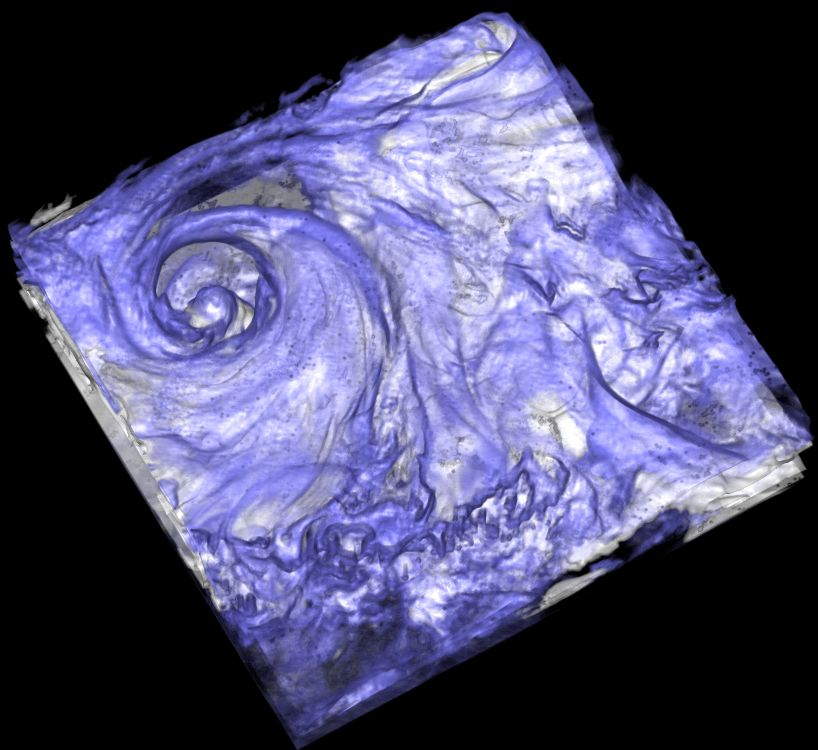
\includegraphics[width=6.5cm, height=4cm, keepaspectratio]{meteorology/humid71f.jpg}}
&
\begin{enumerate}[leftmargin=*, label=\arabic*., topsep=2pt, itemsep=6pt]
    \item Identify the application domain associated with this image. 
    \item What is the dimensionality of the data conveyed in this image? 
    \item What type of visualization technique is used to generate this figure? 
\end{enumerate} \\

\midrule

\nextq & Meteorology
&
\raisebox{-0.9\height}{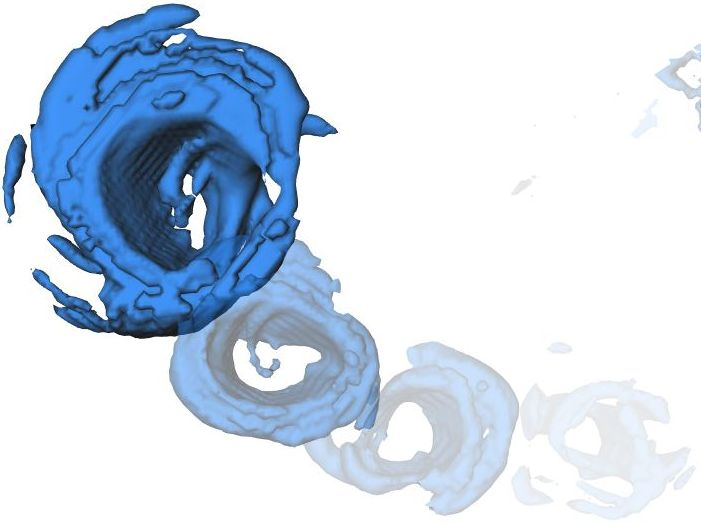
\includegraphics[width=6.5cm, height=4cm, keepaspectratio]{meteorology/opacity_based.jpg}}
&
\begin{enumerate}[leftmargin=*, label=\arabic*., topsep=2pt, itemsep=6pt]
    \item Identify the application domain associated with this image. 
    \item What is the dimensionality of the data conveyed in this image? 
    \item What does the color and opacity represent in this figure? 
\end{enumerate} \\

\midrule

\nextq & Meteorology
&
\raisebox{-0.9\height}{\includegraphics[width=6.5cm, height=4cm, keepaspectratio]{meteorology/meteorology2-handbook.jpg}}
&
\begin{enumerate}[leftmargin=*, label=\arabic*., topsep=2pt, itemsep=6pt]
    \item Locate the the direction of the wind speed on the image. 
\end{enumerate} \\

\midrule


\nextq & Meteorology
&
\raisebox{-0.9\height}{\includegraphics[width=6.5cm, height=4cm, keepaspectratio]{meteorology/thunderstorm-smaller.png}}
&
\begin{enumerate}[leftmargin=*, label=\arabic*., topsep=2pt, itemsep=6pt]
    \item Identify the application domain associated with this image. 
    \item What is the dimensionality of the data conveyed in this image? 
    \item What type of visualization technique is used to generate this figure? 
    \item Locate the aliasing effect in this figure. 
\end{enumerate} \\

\midrule

\nextq & Astronomy
&
\raisebox{-0.9\height}{\includegraphics[width=6.5cm, height=4cm, keepaspectratio]{astronomy/Bock18OpenSpace2.PNG}}
&
\begin{enumerate}[leftmargin=*, label=\arabic*., topsep=2pt, itemsep=6pt]
    \item Identify the application domain associated with this image. 
    \item What is the dimensionality of the data conveyed in this image?
\end{enumerate} \\

\midrule

\nextq & Astronomy
&
\raisebox{-0.9\height}{\includegraphics[width=6.5cm, height=4cm, keepaspectratio]{astronomy/Bock18OpenSpace4.PNG}}
&
\begin{enumerate}[leftmargin=*, label=\arabic*., topsep=2pt, itemsep=6pt]
    \item Identify the application domain associated with this image. 
\end{enumerate} \\

\midrule

\nextq & Astronomy
&
\raisebox{-0.9\height}{\includegraphics[width=6.5cm, height=4cm, keepaspectratio]{astronomy/Interactive10Costa2.PNG}}
&
\begin{enumerate}[leftmargin=*, label=\arabic*., topsep=2pt, itemsep=6pt]
    \item Identify the application domain associated with this image. 
\end{enumerate} \\

\midrule

\nextq & Uncertainty visualization
&
\raisebox{-0.9\height}{\includegraphics[width=6.5cm, height=4cm, keepaspectratio]{uncertainty/uncertainty-vis2.png}}
&
\begin{enumerate}[leftmargin=*, label=\arabic*., topsep=2pt, itemsep=6pt]
    \item How is uncertainty being represented in the image shown?
\end{enumerate} \\

\midrule

\nextq & Uncertainty visualization
&
\raisebox{-0.9\height}{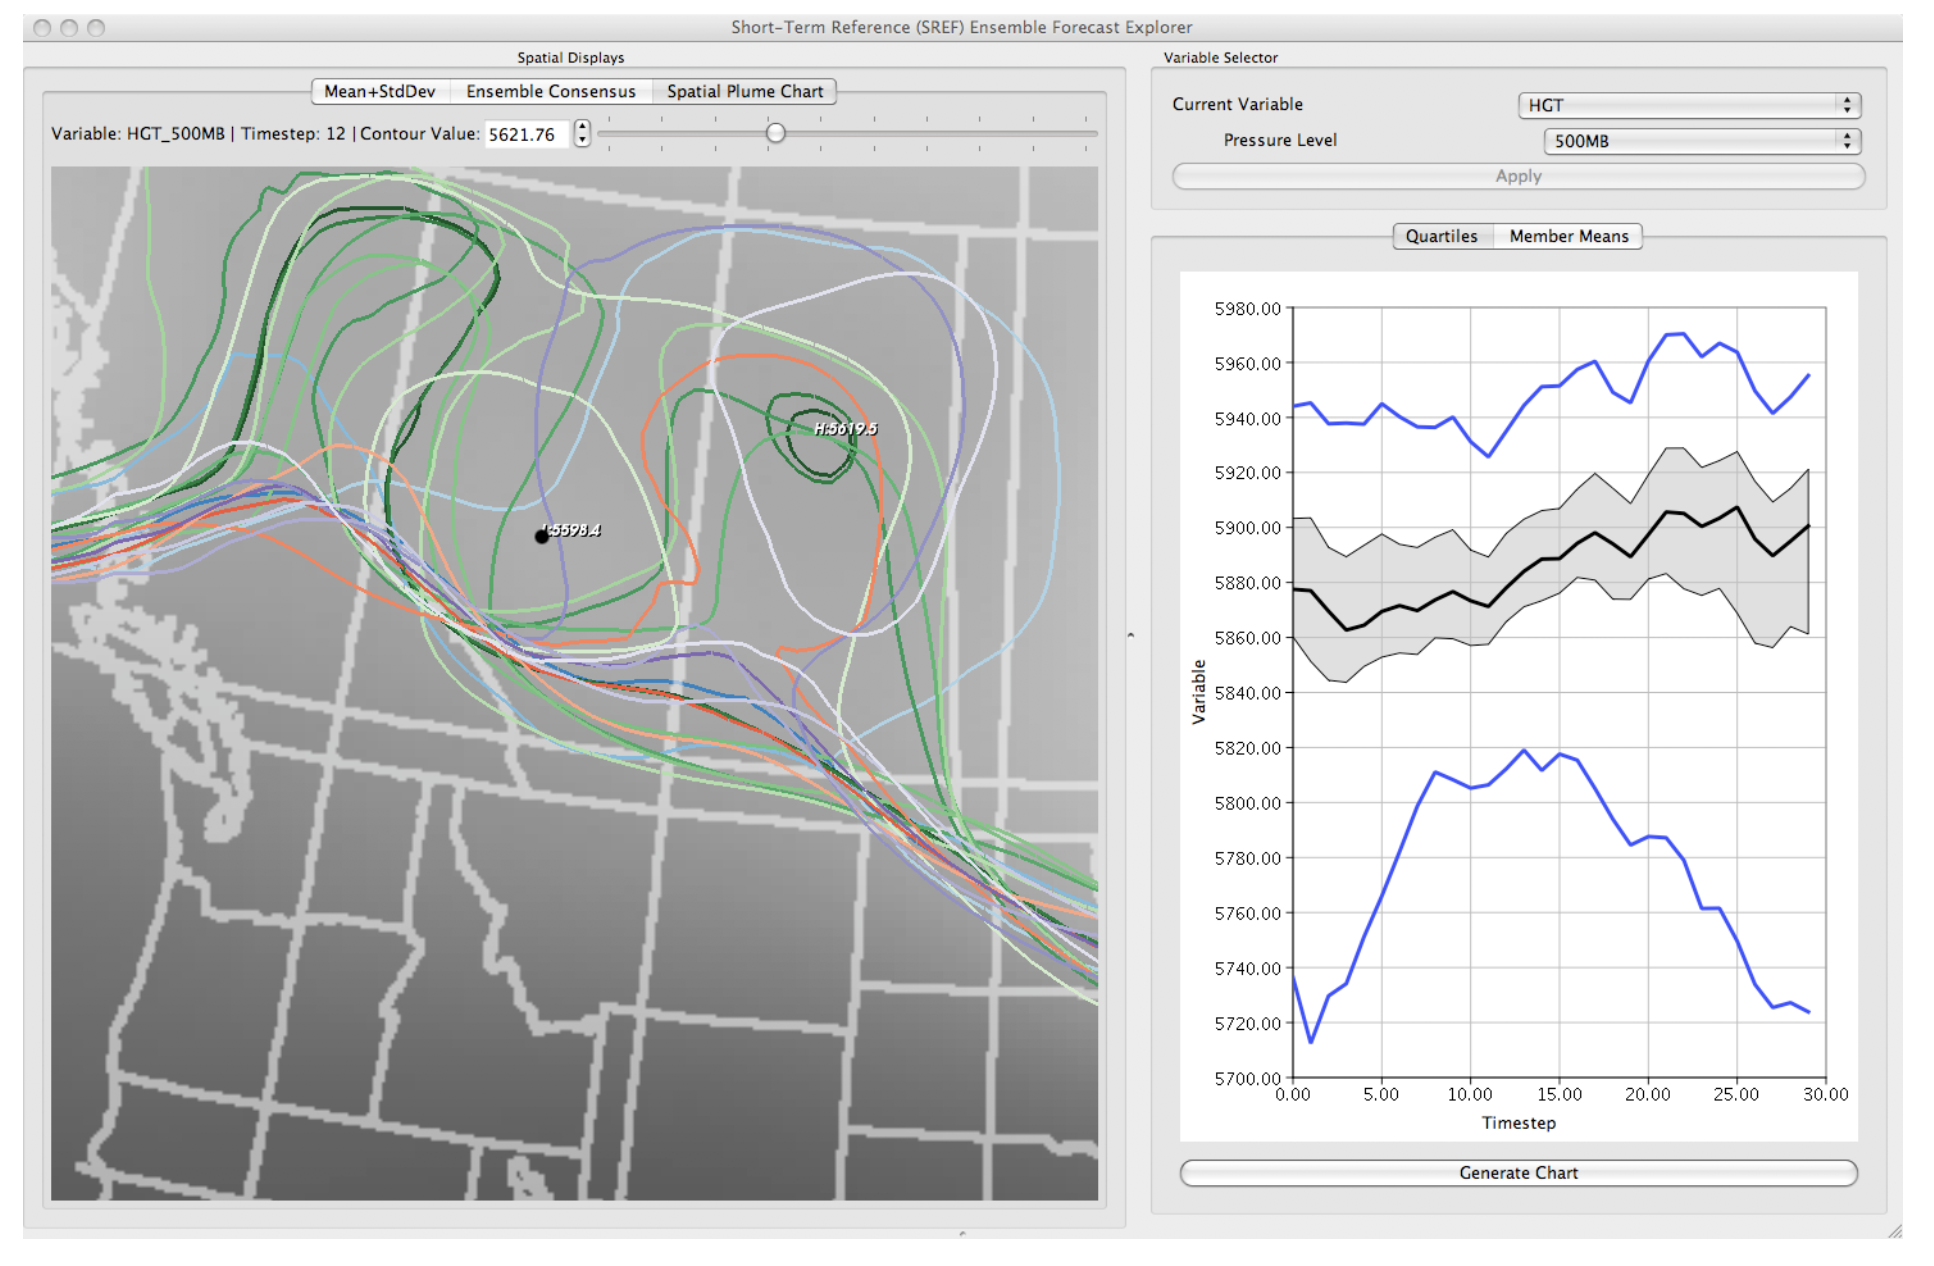
\includegraphics[width=6.5cm, height=4cm, keepaspectratio]{uncertainty/uncertainty-vis1.png}}
&
\begin{enumerate}[leftmargin=*, label=\arabic*., topsep=2pt, itemsep=6pt]
    \item How is the geopotential height being represented using multiple colored lines in this image?
\end{enumerate} \\

\midrule

\nextq & Free Response Questions
&
\raisebox{-0.9\height}{N/A}
&
How would you define an isosurface? \\ 


\midrule

\nextq & Free Response Questions
&
\raisebox{-0.9\height}{N/A}
&
What advantage might glyphs have over streamlines when visualizing flow?\\
    

\midrule

\nextq & Free Response Questions
&
\raisebox{-0.9\height}{N/A}
&
 Why is slicing a useful technique for volume visualization?\\


\midrule

\nextq & Free Response Questions
&
\raisebox{-0.9\height}{N/A}
&
 What is one advantage of a regular grid over an irregular grid?\\
\\

\midrule



\end{longtable}

\end{document}